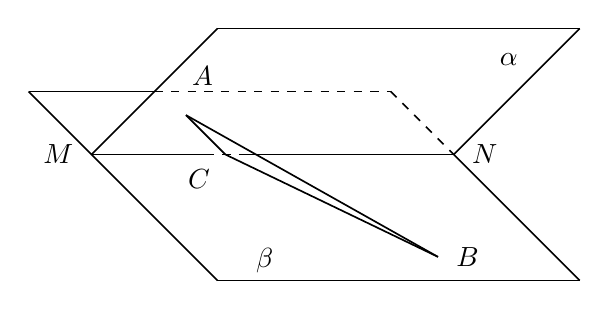
\begin{tikzpicture}[x=1cm,y=1cm,line width=.6pt]
% Planes alpha, beta intersect in MN; triangle ABC with C on MN.
\coordinate (M) at (0,1);
\coordinate (N) at (4.6,1);
\coordinate (C) at (1.7,1);
\coordinate (A) at (1.2,1.5);
\coordinate (B) at (4.4,-0.3);
% upper plane alpha
\coordinate (PA) at (1.6,2.6);
\coordinate (PB) at (6.2,2.6);
\draw (M) -- (PA);
\draw (PA) -- (PB);
\draw (PB) -- (N);
% left extension of alpha top edge
\draw (-.8,1.8)--(M);
\draw (-.8,1.8)--(.8,1.8);
\draw[dashed] (.8,1.8)--(3.8,1.8);
% lower plane beta
\coordinate (QA) at (1.6,-0.6);
\coordinate (QB) at (6.2,-0.6);
\draw (M) -- (QA);
\draw (QA) -- (QB);
\draw (QB) -- (N);
% intersection line MN (small dashed gap at C)
\draw (M) -- (1.45,1);
\draw[dashed] (1.45,1) -- (1.95,1);
\draw (1.95,1) -- (N);
% hidden edge of beta behind alpha (dashed across alpha)
\draw[dashed] (3.8,1.8) -- (N);
% triangle ABC
\draw (A) -- (C);
\draw (C) -- (B);
\draw (A) -- (B);
% labels offset clear of strokes
\node[left,xshift=-3pt] at (M) {$M$};
\node[right,xshift=3pt] at (N) {$N$};
\node[below left,xshift=-2pt,yshift=-2pt] at (C) {$C$};
\node[above,yshift=7pt,xshift=6pt] at (A) {$A$};
\node[right,xshift=3pt] at (B) {$B$};
\node at (5.3,2.2) {$\alpha$};
\node at (2.2,-.35) {$\beta$};
\end{tikzpicture}
